\documentclass[12pt]{report}
\usepackage{graphicx}

\title{SALUTE \\ WEB-BASED MEDICAL MANAGEMENT \\ MILESTONE 0}
\author{Musa Rayyan \\ Nada Hashem \\ Matteo Brucato \\ Ashwin Gopalakrishnan}

\begin{document}
\maketitle
\tableofcontents


\part{Introduction}

\chapter{About this document}

This document is aimed at providing a deep description of the Web-based application that we are developing for the class \emph{CS180 - Introduction to Software Engineering} at the University of California Riverside during the Winter quarter. Our purpose is to provide a documentation that would possibly allow new team members to join the project quickly and easily. At the same time this documentation will help us to keep an audit trail of what we did and how we did it. We will discuss all our researches, problems and decision.

The report is divided into 5 parts. The first one comprises this brief introduction along with an overview of the system we designed and implemented. The second part is a list of all the requirements needed, whereas the third part is a high-level view of the system, i.e its design and a low-level description, i.e. its implementation. Then, we added an operating manual for the end-user and a section for credits and acknowledgements.

\chapter{Overview}
Our application is a web-site, running through https (secure http), to manage patient's healthcare documents and resources. The logic and behaviour is centred on patients, rather than on Health Care Providers. In this view, all HCPs are considered as ''customers'' of patients. Patients can ask for ''social connections'' with HCPs, can upload or download their medical records and grant access to them to a specific set of doctors. They can also manage their appointments and bills.

\section{Description/Motivation}
We quote here the entire description given in the requirement paper for Milestone 0. We believe that this gives the best perspective in order to understand the whole system.
\begin{quotation}
   Modern medical offices rely on specialized software to manage the care and treatment of patients. Often,
such software “locks” data into a proprietary format and/or behind excessive security protocols. These
measures prevent the easy flow of information between patients and their doctors. As case in point, a
patients medical records are often seen as the “property” of the health care provider rather than the patients
personal property.
   
   The objective of this project is to create a web-based medical management portal in which a patient retains
control over their own medical records, yet provides easy access to any authorized healthcare provider. This
project is envisioned as part social network, part medical information database that will allow for patient
authorized “sharing” of relevant medical records to various doctors and specialists.
   
   This application will provide a web-based health information portal for (at least) two distinct groups
(patients and doctors). A patient will be allowed to create and manage their own profile, view and manage
their medical records, create and withdrawal “sharing links” to their selected health care providers, and
schedule/request appointments. Doctors will have a patient management service that will allow for the
scheduling/authorizing appointments, managing patient care, and billing functionality.
\end{quotation}


\chapter{Tools and Technology}
We immediately realized that the best way to implement a complex Web application like \emph{Salute} was using all the possible technologies that we were aware of. Firstly, we decided to use a well-known system design such as \emph{MVC} (Model-View-Controller). We also decided to use a framework named \emph{CodeIgniter}\footnote{www.codeigniter.com} that is written in Php\footnote{www.php.net}. We fixed \emph{LAPP} as our system environment stack. LAPP stands for \emph{Linux}, \emph{Apache}, \emph{PostgreSQL}, \emph{Php}. Then we decided to use \emph{XHTML} as a markup language to describe web pages because it is standardized and is an XML, and use a Javascript framework called \emph{JQuery}\footnote{www.jquery.com} to have a powerful set of tools that are easy to use and browser-independent. In order to separate the concern of "what to display" and "how to display it", we decided to use \emph{CSS} to manage layouts and presentational matters in the interface. We also decided to foresee the change and implemented Ajax natively.

We chose \emph{Doxygen}\footnote{www.doxygen.com} as a parsable-formalized way to write comments in the code. Doing so, we were able to create a detailed documentation for the implementation, automatically,

Last but not least, we decided to use \LaTeX as the language and tool for writing the documentation.

This is just a brief introduction to the tools and technologies that we used in our project. We will go into more details in the rest of this documentation.


\part{Requirements}
\chapter{User Requirements}
The user requirements presented by the client can be categorized into general, patient side, and healthcare provider side requirements.

\section{General}
\begin{itemize}
\item A patient or healthcare provider should be able to crate, delete, and modify their respective account
\item Accounts should be protected by a username and password combination
\item Depending on the type of user account, each user will have a unique user profile within the system
\item Depending on the type of user account, one of two social networking connection options are available. When requesting a social network connection, proper confirmation is required.  Upon forming a social network connection, the patient and provider will be listed in each other's respective list of contacts.
\begin{itemize}
\item (Patient to Healthcare Provider) This type of connection can only be requested by a patient and represents the "doctor-patient" relationship.  When this connection is formed, it allows the provider access to the patient's medical records and indicates a level of trust between the patient and healthcare provider.
\item (Healthcare Provider to Healthcare Provider) This relationship only exists between providers and represents the providers network of health care professionals.
\end{itemize}
\item Under each user's account, the list of their current contacts will be readily available and linked to their respective profile pages
\item Medical records may be uploaded by a patient or a healthcare provider that is connected to that patient
\end{itemize}

\section{Patient side}
\begin{itemize}
\item Patient accounts are exclusively for the use of patients
\item A patient account may only be allowed to connect with a healthcare provider acccount
\item No patient information will be available to other patient accounts
\item Patient information is only available to healthcare providers to which the patient is connected with
\item May organize their medical records
\item May manage their privacy settings
\item May connect, message, and interact with their healthcare providers
\end{itemize}

\section{Healthcare Provider Side}
\begin{itemize}
\item Healthcare provider accounts are exclusively for the use of healthcare providers
\item A healthcare provider account may connect with either patient accounts or other healthcare provider accounts (specialists or colleagues)
\item May view a listing of all their patient contacts
\item May view the available medical records of an individual patient
\item May schedule appointments
\item May message, interact and connect with patients and other healthcare providers
\end{itemize}

\chapter{System Requirements}
The system requirements are as follows:
\begin{itemize}
\item The system will be web-based
\item The user will interact with the server through a web brower
\item The server will be web-based, using an appropriately selected web server to handle communication requests.
\item The brower must be able to handle communication with the webserver using https (secure http)
\item The server will only communicate with the client interface over https.  All other connections will be automatically switched to https.
\item The server will maintain a list of cantacts for each user
\item The server must be able to receive copies of the patients medical records
\item All necessary system data will be stored in an appropriately selected and designed database, capable of interacting with the server.
\item The user interface must be able to upload files to the server
\end{itemize}

\chapter{Current Status and Future Work}
\paragraph{Messaging} Currently it is implemented by using users' existing email addresses, and emailing via the website. We have already implemented the messages table in the database in case for future interests to have our own messaging system.

\part{Design}

\chapter{High Level View}
Bla bla bla..

\section{System Design}
A Web application can be simplified as a collection of resources placed on a server which are accessible to a great number of users (clients). The access to these resources must be governed by policies and permissions. From a very general point of view, our application has two kinds of resources: \emph{public} and \emph{private} resources. For instance, the login page must be a public resource, whereas the setting page should be private.

You can think of a resource as either some data inside a database, a functionality that you ask to your application or even the result of some kind of operation. Based on this view, we decided to use a well-known design approach called MVC (Model-View-Controller) that works very well with this kind of settings. A controller is some executing code that performs exactly the action that the user asked to the server via an URL. In this way, a URL becomes the medium to ask for functionalities and a controller will be a merely executor. A model will be the medium to access data into a database and a view will be a result for the user, in a interface-depending fashion.

In this chapter we will describe our design from a high-level viewpoint, living the implementation for the next chapter.

\section{Database Design}
Bla bla bla... general description ... why we chose to implement it like this... what problems we faced... etc...

\subsection{Entity Relationship Diagram (ERD)}
We provide a high-level description of the database using the famous ER diagram, for those who are familiar with it\footnote{Entities are represented in the ER diagram as rectangles.  Each entity represents a table in the database that holds all of the information or attributes that represents that entity.  In the ER diagram, each attribute is represented with a oval.}. Then we will describe the database structure in more details.

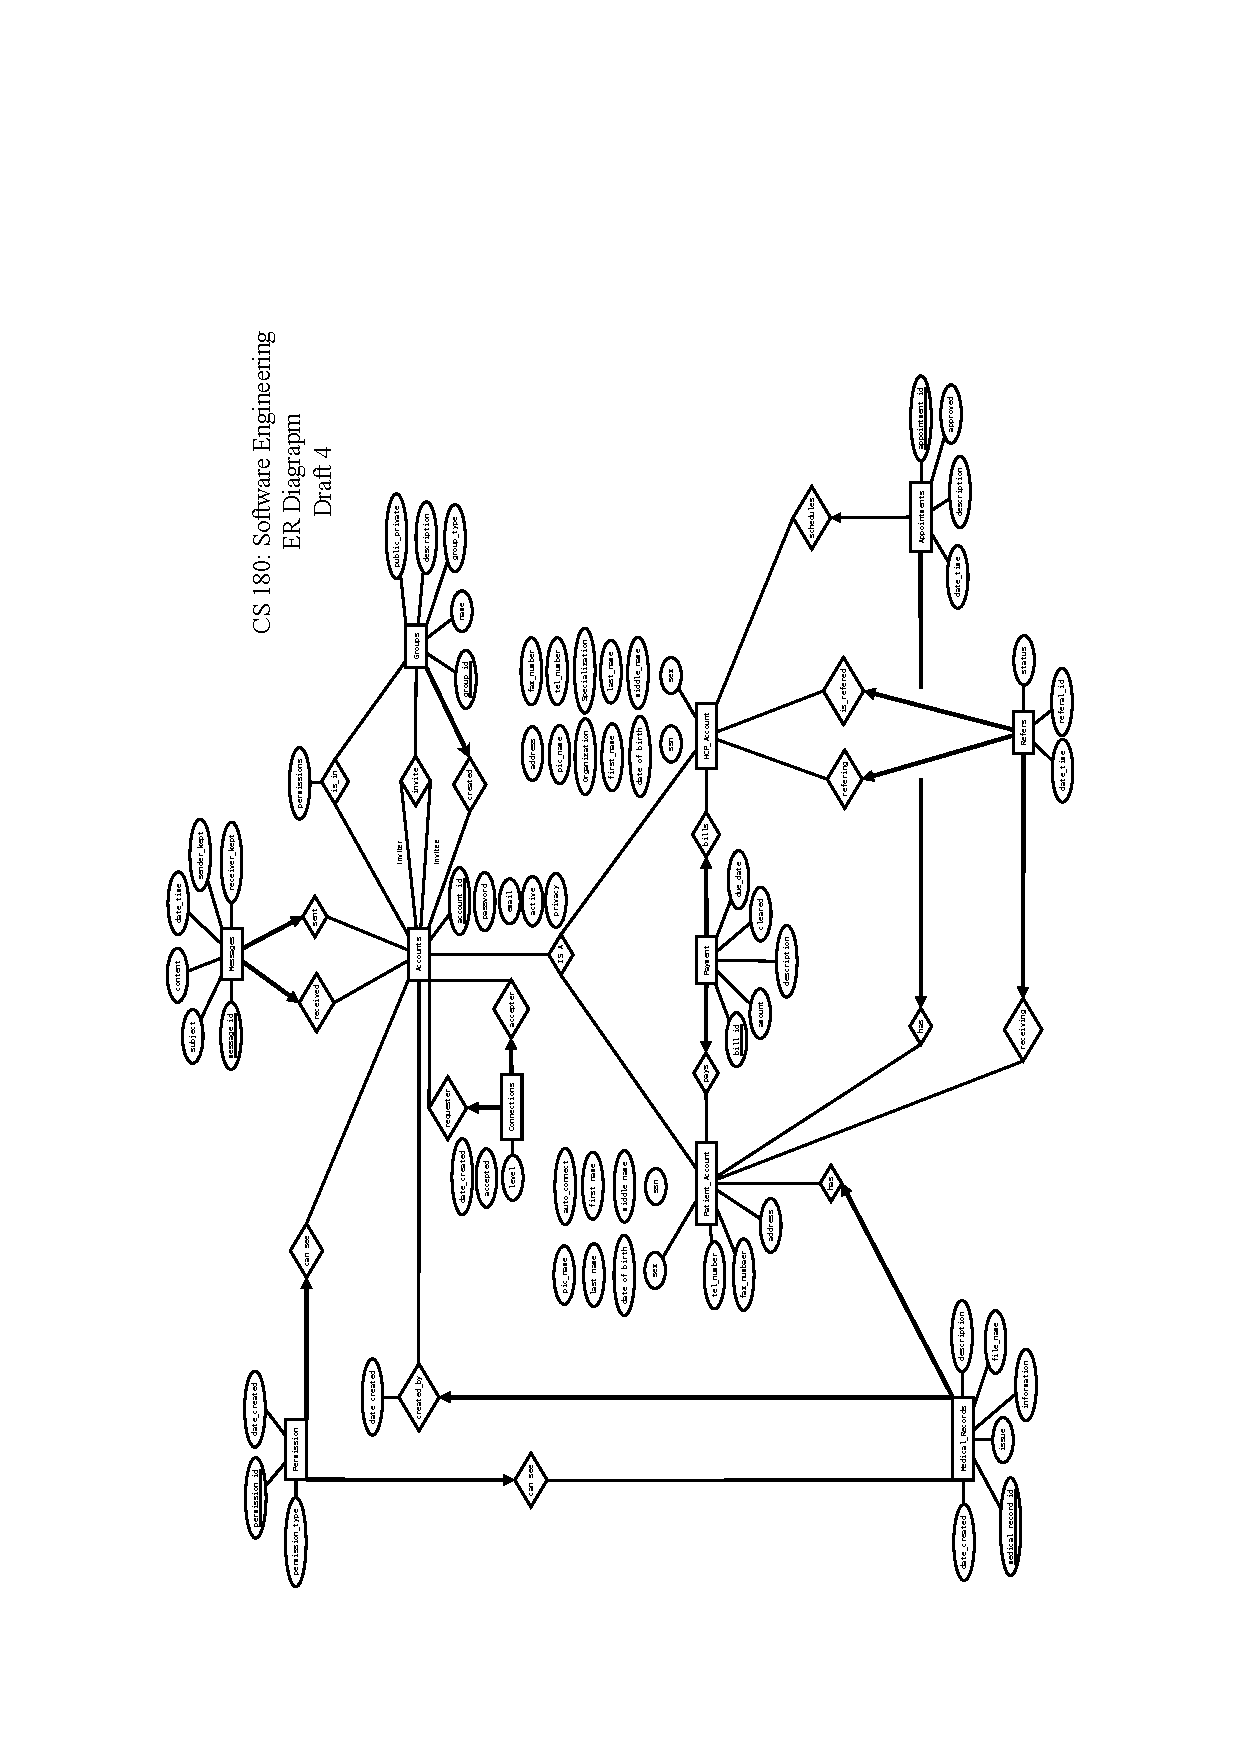
\includegraphics[scale=0.6,angle=180]{cs180_ER_draft4.pdf}

\section{MVC Design}

MVC stands for Model View Controller, and is a software architecture and an architectural pattern in software engineering. The purpose is to separate a system into parts,assigns responsibilities to each, and ensures that they can work together. This design method strives for high cohesion and low coupling which is essential in anticipating for future changes. There are several frameworks that follow this paradigm, such as Ruby on Rails, ASP.net, and CodeIgniter. We used CodeIgniter to aid the design of Salute, our product.  

\subsection{Controllers}

The controller is the middle man. It's in charge of loading the view(webpage) for the user, and calling the corresponding models to execute the functionality that the user has selected via the view. 
It is good practice to separate control into several controllers for separation of concerns. In our product Salute,the controllers were separated in this way\footnote{See MVC implementation 7.2.1}. Notice that many of these controllers depend on the fact that the user is logged in as a member of Salute. While many controllers depend on this Home Controller functionality for handling login and logout, this relation is minimal (low coupling) since we used a CodeIgniter's session class. This separated the concern of user authorization out from other controllers. 
Also note that all the functions within a controller access, view, or modify the same elements of information(high cohesion). This division bewteen controllers allows for general flexibility and ease to adding, removing, or modifiying more functions in the future. If a whole new feature, e.g. diet log, is later decided to be added to Salute, a new controller can be created, and little to no changes would need to be made to the existing controllers. 
\subsection{Models}
The model is the tool used to access and modify the database. Everytime a user needs information, the models are queried to retrieve the information. If a user wants to add or modify, this too must be added into the database. The results are then returned to the controller for further action.
Models too are separated based on functionality. This separation correlates closely to how the database is implemented, and what the controller needs from the database\footnote{See MVC implementation 7.2.1}. This separation also accomodates for change. If a new feature is added to appointments, e.g. send email reminder 3 days before appointment, a new model function within the Appointments model can be written to retrieve such appointments for the controller to carry out this new feature. 

\subsection{Views}
The view is the the user interface, what the user sees and interacts with. In our case, its a medical management website. So, it is important to make sure that the website is user-friendly. If the layout and design of the view is difficult to navigate and/or inconsistent, the user will not desire to use the product. The views are called by the controller, and take user input and send it back to the controller to manage what action needs to be done. 
Our product, Salute, divided the views into two main subcategories: main panel, and side panel. The main panel views are all the views that are called to be in the main panel of the screen. The side panel views are all the views that are called to be in the side panel. There are multiple views in each of these subcategories since each functionality needs a different display, and often functionalities differ based on the type of user(a non-member,a patient, or a healthcare provider). 

\section{Interface Design}
Since this is a Web application, the interface is basically a set of HTML pages that a client gets from the server as it requests them. As for every Web page, the interface is a mixture between different technologies, like HTML, CSS, Javascript and so forth. It is also dependant in some degree by some server features. To keep everything simple, the interface design only defines a very high view of the user system. To allow for a better separation of concerns, we also divided the ''content'' of the Web page from the ''presentation'' of it.
\subsection{UI design}
The GUI is composed by:
\begin{itemize}
\item a header
\item a navigation bar
\item a footer
\item two \emph{dynamic} panels
	\begin{itemize}
	\item a main panel to display the main content of the page
    \item a side panel to display additional information about the main content
	\end{itemize}
\end{itemize}
The header basically contains the branding. The navigation bar allows a user to navigate between all the \emph{public} resources of the entire application and the footer has an extra set of public resources, not directly related to the use of the Web site.

The two panels are \emph{dynamic} in the sense that their content depends on the current resource the user is accessing on a particular moment. They change during the application use, request after request.

\subsection{Ajax}
To follow a generic principle in Software Engineering, we decided to anticipate the change, creating our system capable to do every request using the famous technology Ajax. To be more precise, using requests to server called XMLHTTPRequest. Our interface is ready for that change, and the two dynamic panels are the ones that would change after a XHR request. Both the client and the server are aware of this and whenever the server receives an XHR request, it will answer with only the content for the two dynamic panels. Whereas, if the request is a normal HTTP request, it will provide the whole interface to the client. We will discuss later how we implemented it.

\subsection{Layout}
It's really hard to set a limit between content and presentation in an environment governed by HTML, but something can be done. We created all our views regardless of presentation aspects, focusing only on the most simple aspects of HTML. Our purpose is to separate this two concerns and leave to the \emph{layout} the task to add colours, change positions of the elements and this kind of things. Doing so we also provided the possibility to change the layout in the future, or even dynamically.

\section{Server Design}



\chapter{Implementation View}
This chapter will show in more details how we implemented all the requirements using the design that we discussed in the previous chapter. We will show the full database, MVC, interface and server implementation, along with a list of all the assumptions that we made during the development phase. We will also present a list of the tests that we made.

\section{Database implementation}
\subsection{Tables}
Our database is composed of ten tables: Messages, Accounts, Patient\_Account, HCP\_Account, Appointments, Medical\_Record, Payment, Permission, P\_D\_Connection, and D\_D\_Connection.  For each table, we will present a descryption of the table and the attributes in it, as well as its relationship with the other tables its connected with.

\subsubsection{Messages}
Holds all of the information regarding messages sent from patient to hcp or vice versa. It has two total 1:N relationships with the Accounts entity.

\begin{description}
\item serial \textit{message\_id}- ID to uniquely identify the message from other messages. serial datatype automatically creates the message\_id when a new tuple is inserted into the table.  Primary key of the table.  Cannot be null.
\item text \textit{subject}- Subject of the message being sent. text datatype allows unlimited number of characters.  Cannot be null.
\item text \textit{content}- Where the sender can writte what they would like to send to the receiver.  text datatype allows unlimited number of characters.  Cannot be null.
\item serial \textit{message\_id}- ID to uniquely identify the message from other messages. serial datatype automatically creates the message\_id when a new tuple is inserted into the table.  Primary key of the table.  Cannot be null.
\item timestamp \textit{date\_time}- Date and time of when the message is sent.  timestamp datatype format YY:MM:DD HH:MM:SS.  Cannot be null.
\item boolean \textit{sender\_kept}- To determine if the sender would like to delete the message from their outbox.  boolean value is either true or false.  Cannot be null.  By default it is true.  Changing the status to false means it gets deleted.
\item boolean \textit{receiver\_kept}- To determine if the receiver would like to delete the message from their inbox.  boolean value is either true or false.  Cannot be null.  By default it is true.  Changing the status to false means it gets deleted.
\end{description}

\subsubsection{Accounts}
Holds all of the primary information every patient and hcp account needs to log into Salute.  The entities Patient\_Account and HCP\_Account both inherit from Accounts using an IS A relationship.  It has a partial N:1 relationship with the Permission and Medical\_Records entities.

\begin{description}
\item serial \textit{account\_id}- ID to uniquely identify the account from other accounts. serial datatype automatically creates the account\_id when a new tuple is inserted into the table.  Primary key of the table.  Cannot be null.
\item varchar(40) \textit{email}- Email of the account holder. It is used to log into Salute along with the user password.  varchar(40) datatype allows for a maximum of 40 characters.  Cannot be null.
\item varchar(15) \textit{password}-  Password of the account holder.  It is used to log into Salute along with the user email address.  varchar(15) datatype allows for a maximum of 15 characters.  Cannot be null.
\item boolean \textit{active}- To determine wheather the account is active or not.  boolean datatype value is either true or false.  By default it is true.  Changing the stauts to false means the account gets deactivated.
\end{description}

\subsubsection{Patient\_Account}
Holds all of the personal information for every patient.  It inherits from the Accounts entity with an IS A relationship.  It has a partial N:1 relationship with the Medical\_Records entity and a partial N:M relationship with the p\_d\_connection relationship.

\begin{description}
\item serial \textit{account\_id}- ID to uniquely identify the account from other accounts. serial datatype automatically creates the account\_id when a new tuple is inserted into the table.  This ID is inherited from the Accounts entity. Primary key of the table.  Cannot be null.
\item varchar(30) \textit{first\_name}-  First name of the patient.  varchar(30) datatype allows for a maximum of 30 characters.  Cannot be null.
\item varchar(30) \textit{last\_name}- Last name of the patient.  varchar(30) datatype allows for a maximum of 30 characters.  Cannot be null.
\item varchar(30) \textit{middle\_name}- Middle name of the patient. varchar(30) datatype allows for a maximum of 30 characters.
\item numeric(9,0) \textit{ssn}- Social Security Number of the patient. numeric(9,0) datatype allows exactly 9 numeric characters.  Cannot be null.
\item date \textit{dob}- Date of Birth of the patient.  date datatype is of the format YY:MM:DD.  Cannot be null.
\item char(6) \textit{sex}- Sex of the patient. char(6) datatyep allows for a maximum of 6 characters.  It has to be either "male" or "female".  Cannot be null.
\item varchar(11) \textit{tel\_number}- Primary telephone number of the patient.  varchar(11) datatype allows a maximum of 11 characters.
\item varchar(11) \textit{fax\_number}- Fax number of the patient.  varchar(11) datatype allows a maximum of 11 characteres.
\item text \textit{address}- Primary address of the patient.  text datatype allows unlimited number of characters.
\end{description}

\subsubsection{HCP\_Account}
Holds all of the personal information for every hcp.  It inherits from the Accounts entity with an IS A relationship.  It has a partial N:1 relationship with the Appointments and Payment entities, as well as a partial N:M relationship with the p\_d\_connection and d\_d\_connection relationship.

\begin{description}
\item serial \textit{account\_id}- ID to uniquely identify the account from other accounts. serial datatype automatically creates the account\_id when a new tuple is inserted into the table.  This ID is inherited from the Accounts entity. Primary key of the table.  Cannot be null.
\item varchar(30) \textit{first\_name}-  First name of the hcp.  varchar(30) datatype allows for a maximum of 30 characters.  Cannot be null.
\item varchar(30) \textit{last\_name}- Last name of the hcp.  varchar(30) datatype allows for a maximum of 30 characters.  Cannot be null.
\item varchar(30) \textit{middle\_name}- Middle name of the hcp. varchar(30) datatype allows for a maximum of 30 characters.
\item numeric(9,0) \textit{ssn}- Social Security Number of the hcp. numeric(9,0) datatype allows exactly 9 numeric characters.  Cannot be null.
\item date \textit{dob}- Date of Birth of the hcp.  date datatype is of the format YY:MM:DD.  Cannot be null.
\item char(6) sex- Sex of the hcp. char(6) datatyep allows for a maximum of 6 characters.  It has to be either "male" or "female".  Cannot be null.
\item varchar(11) \textit{tel\_number}- Primary office telephone number of the hcp.  varchar(11) datatype allows a maximum of 11 characters.
\item varchar(11) \textit{fax\_number}- Primary fax number of the hcp.  varchar(11) datatype allows a maximum of 11 characteres.
\item text \textit{specialization}- What the hcp specializes in.  text datatype allows unlimited number of characters.
\item varchar(30) \textit{org\_name}- Name of the organization for which the hcp works for.  varchar(30) datatype allows a maximum of 30 characteres.
\item text \textit{address}- Primary address of the hcp place of business.  text datatype allows unlimited number of characters.
\end{description}

\subsubsection{Appointments}
Holds all of the information for every appointment a patient makes with a hcp.  It has a total 1:N relationship with the HCP\_Account and Patient\_Account entities.

\begin{description}
\item serial \textit{appointment\_id}- ID to uniquely identify the appointment from other appointments. serial datatype automatically creates the appointment\_id when a new tuple is inserted into the table.  Primary key of the table.  Cannot be null.
\item serial \textit{patient\_id}-  Unique account ID of the patient that requests the appointment.  This is the foreign key to the Patient\_Account entity.  Cannot be null.
\item serial \textit{hcp\_id}- Unique account ID of the hcp that receives the appointment request.  This is the foreign key to the HCP\_Account entity.  Cannot be null.
\item text \textit{descryption}- Description of the appointment that the patient requests to the hcp.  text datatype allows unlimited number of characters.  Cannot be null.
\item timestamp \textit{date\_time}- Time and day of the appointment the patient requestes to the hcp.  timestamp datatype of the form YY:MM:DD HH:MM:SS.  Cannot be null.
\item boolean \textit{approved}- Status of the appointment that the patient requests to the hcp.  boolean datatype value is either true or false.  By default it is false.  HCP can accept the appointment and change the status to true.
\end{description}

\subsubsection{Medical\_Record}
Holds all of the information for every medical record a patient has on Salute.  It has a partial N:1 relationship with the Permission entity and a total 1:N relationship with the Accounts and Patient\_Account entities.

\begin{description}
\item serial \textit{medical\_rec\_id}- ID to uniquely identify the medical record from other medical records. serial datatype automatically creates the medical\_rec\_id when a new tuple is inserted into the table.  Primary key of the table.  Cannot be null.
\item serial \textit{patient\_id}- Unique account ID of the patient that owns the medical record.  This is the foreign key to the Patient\_Account entity.  Cannot be null.
\item serial \textit{account\_id}- Unique account ID of the user(patient/hcp) that uploads the medical record.  This is the foreign key to the Accounts entity.  Cannot be null.
\item text \textit{issue}-  What the medical record deals with.  text datatype allows unlimited number of characters.  Cannot be null.
\item text \textit{suplementary\_info}- Any suplementary infomation that anybody (patient/hcp) would want to add to the medical record.  text datatype allows unlimited number of characters.
\item text \textit{file\_path}- Path where the file can be found and downloaded from the server.  text datatype allows unlimited number of characters.  Cannot be null.
\end{description}

\subsubsection{Payment}
Holds all of the information for every bill that a patient receives and a hcp issues.  It has a total 1:N relationship with the Patient\_Account and HCP\_Account entities.

\begin{description}
\item serial \textit{bill\_id}-  ID to uniquely identify the bill from other bills. serial datatype automatically creates the bill\_id when a new tuple is inserted into the table.  Primary key of the table.  Cannot be null.
\item serial \textit{patient\_id}- Unique account ID of the patient that received the bill.  This is the foreign key to the Patient\_Account entity.  Cannot be null.
\item serial \textit{hcp\_id}- Unique account ID of the hcp that issued the bill.  This is the foreign key to the HCP\_Account entity.  Cannot be null.
\item decimal(9,2) \textit{amount}- The amount due to the hcp.  decimal datatype allows charge to be up to 9 digits long, with 2 digits of percision.  Cannot be null.
\item text \textit{descryption}- Descryption of what the bill is being issued for.  text datatype allows unlimited number of characters. Cannot be null.
\item timestamp \textit{due\_date}- Date by which the bill must be paid by.  timestamp datatype of the form YY:MM:DD HH:MM:SS.  Cannot be null.
\item boolean \textit{cleared}- States wheather the bill was paid or not.  boolean datatype value is either true or false.  By default it is false.  If patient pays the bill, its status is changed to true.
\end{description}

\subsubsection{Permission}
Holds information regarding which medical records a hcp that is connected with a patient can view.  It has a total 1:N relationship with the Accounts and Medical\_Records entities.

\begin{description}
\item serial \textit{permission\_id}-  ID to uniquely identify the permission from other permissions. serial datatype automatically creates the permission\_id when a new tuple is inserted into the table.  Primary key of the table.  Cannot be null.
\item \textit{medical\_rec\_id}- Unique ID of the medical record that a hcp can view.  This is the foreign key to the Medical\_Records entity.  Cannot be null.
\item serial \textit{account\_id}- Unique ID of the hcp that can view the medical record.  This is a foreign key to the Accounts entity.  Cannot be null.
\item date \textit{date\_created}-  Date in which the patient allowed the hcp to view the medical record.  date datatype is of the form YY:MM:DD.  Cannot be null.
\end{description}

\subsubsection{p\_d\_connection}
Holds all of the information for every connection between a patient and a hcp.  This relationship has a patial N:M relationship with the HCP\_Account and the Patient\_Account entities.

\begin{description}
\item serial \textit{patient\_id}- Unique account ID of the patient that establishes a connection with a hcp.  The combination of patient\_id and hcp\_id is the primary key for this table.  This is also the foreign key to the Patient\_Account entity.  Cannot be null.
\item serial \textit{hcp\_id}- Unique account ID of the hcp that accepts the connection request sent from the patient.  The combination of hcp\_id and patient\_id is the primary key for this table.  This is also the foreign key to the HCP\_Account entity.  Cannot be null.
\item boolean \textit{accepted}- States wheather the request was accepted by the hcp.  boolean datatype value is either true or false.  By default it is false.  If hcp accepts the request, its status is changed to true.
\item date \textit{date\_connected}- Date in which the request was sent by the patient to the hcp.  date datatype is of the form YY:MM:DD.  Canot be null.
\end{description}

\subsubsection{d\_d\_connection}
Holds all of the information for every connection between a hcp and another hcp.  This relationship has two patial N:M relationships with the HCP\_Account entity.

\begin{description}
\item serial \textit{requester\_id}- Unique account ID of the hcp that establishes a connection with another hcp.  The combination of requester\_id and accepter\_id is the primary key for this table.  This is also a foreign key to the HCP\_Account entity.  Cannot be null.  
\item serial \textit{accepter\_id}- Unique account ID of the hcp that accepts the connection request sent from hcp.  The combination of accepter\_id and requester\_id is the primary key for this table.  This is also a foreign key to the HCP\_Account entity.  Cannot be null.
\item boolean \textit{accepted}- States wheather the request was accepted by the hcp.  boolean datatype value is either true or false.  By default it is false.  If hcp accepts the request, its status is changed to true.
\item date \textit{date\_connected}- Date in which the request was sent by the hcp to the other hcp.  date datatype is of the form YY:MM:DD.  Canot be null.
\end{description}

\subsubsection{Scripts to start the server and load the data}
We used many scripts to create the database described above.  First of all we have a bash script called start\_everything.sh which as its name implies, starts everything.  It starts the PostgreSQL server, creates a PostgreSQL database, and then it uses an sql file called create\_tables.sql to create all of the tables described in the ER diagram.  It then calls the file load\_data.sql which loads all of the tables with test data.  In case we want to drop all of the test data we have an sql file called drop.sql.  In case we wanted to delete everything and start over, we have a bash script called delete\_everything.sh. 

\section{MVC implementation}
In this section we will provide detailed, low-level information about the MVC that we implemented. Secondly, we list all the important assumptions that we made, that are fundamental for the understanding of the system.

\subsection{Doxygen documentation}
All the models, views and controllers have been implemented incorporated into the CodeIgniter framework in Php. We used the Doxygen\footnote{www.doxygen.org} comment format to be able to create a complete and organized implementation documentation out of the comments. For this reason, all the documentation for the MVC is into a separate document called \emph{Salute - MVC Implementation}. There one can find all the necessary details, together with a list of ''todo's'', a list of ''tests'' and a list of ''bugs''.

\subsection{Assumptions}
We made these remarkable assumption during the implementation of the MVC.
\begin{itemize}
\item Doctors cannot delete medical records even if they uploaded them, only patients can
\item Both doctors and patients can upload medical records
\item When a doctor uploads a medical record, he has automatic viewing priveleges
\item doctors cannot request appointments
\item patients cannot accept an appointment
\item doctors aren't allowed to reschedule an appointment
\item both doctors and patients can cancel an appointment
\end{itemize}

\section{Interface implementation}
In the design description we gave a high-level view of the interface, without going into details. We have seen that the UI is composed by tree 'fixed' components and two 'dynamic' components. Now we will show how those components all fit together into an actual code and how server and client are aware of the interface and can interact with it.

\subsection{Layouts}
A layout, as we believe, is just a way to reorganize spatially the content of a web page. Since all the XHTML content is provided to the client without any presentational description, a page without a layout would be a simple flow of objects (text, lists, tables and images) in cascade.

We used CSS to create a layout out of an XHTML document. We also used some Javascript when we wanted to add some other features to that layout. For example, you can see that every page is showed gradually and smoothly when loaded.

\paragraph{Layout folder}
All layouts styles are contained into the folder /layouts. This contains a specific folder for each specific layout. At this moment of implementation we have one layout called ''faux-8-2-col''\footnote{We used a free css layout from http://www.code-sucks.com/css\%20layouts/}. Inside its folder you can see all the .css and .js files necessary to describe \emph{position}, \emph{color}, \emph{size} and so forth, of every object in the XHTML page. It's also the layout that decides whether using Ajax or not, because we believe that the XHR functionality is a layout matter.

\paragraph{Template XHML files}
For each of these folders there is a specific XHTML template file that organize the five components of the interface into an XML tree. These files are contained into the folder
\begin{verbatim}
/system/application/views/layouts
\end{verbatim}
Every template file contains the five interface components: 'header', 'navbar', 'mainpane', 'sidepane' and 'footer'. We decided to use the template parser provided by CodeIgniter, so that the XHTML contains only references to these components.


\paragraph{Server Layout management}
On the server side, all the logic for the layout has been implemented in the class \begin{verbatim}/system/application/libraries/layout.php
\end{verbatim}
This class contains all the possible layouts. There is a method to set the current layout and a method get all the XHTML for the current layout. This method only needs an array with two elements: a string to put inside the 'mainpane' and another one to put inside the 'sidepane' of the interface, as we already discussed. Then, it will simply call the CodeIgniter template parser to insert all the content into the template.

\paragraph{JQuery}
We use JQuery for at least three reasons: provide 'fancy' effects to the page, implement some client checks on forms and make Ajax requests. JQuery is a framework for Javascript that makes all of these features easy to implement.

\subsection{Ajax interaction between client and server}
It is clear that if the client does an XMLHTTPRequest the server should be aware of this, and answer correctly. This is what this class does
\begin{verbatim}/system/application/libraries/ajax.php
\end{verbatim}
It checks whether the request has been received via XHR (Ajax) or not. If the request was made using XHR, the method view() will then send to the client only the dynamic content, i.e. the 'mainpane' and the 'sidepane'. Otherwise, it will call the layout class to get the whole interface and send it to the client. It takes an array with two strings: the content for the mainpane and the content for the sidepane.

In case of an Ajax response, it will be encapsulated into a JSon array. This class also handles redirections. In case of a redirection via Ajax, a specific element with name 'redirect' will be inserted into the JSon array, containing the URL to redirect to.

\subsection{Interaction between Controllers and Layout/Ajax}
All the controllers will create their views into two strings, one for the 'mainpane', the other for the 'sidepane'. At the end of their computation they will call the class 'Ajax', passing those two strings, in order to send a response back to the client.


\section{Authorization}
We already mentioned how the login phase works. In this section we will show in details how we use http cookies to memorize the authorized state of clients.
\subsection{Session cookie}
After a client successfully logs in (after its e-mail and password match a row in the database), a session cookie is created. This cookie will contain this information:
\begin{itemize}
\item The account\_id of the user
\item The type of the user (either 'patient' or 'hcp')
\item The email of the user
\item His/her first name
\item His/her last name\footnote{First name and last name may not be useful if we decide to change the definition of HCPs to 'group of people' instead of individuals. But this would require a little change only in the database and its model. The session cookie may have these two fields empty, or add extra fields.}
\end{itemize}
We also used a functionality in CodeIgniter, to save the session\_id into a special table in the database. Those tuples will be handled automatically by CodeIgniter every time a user creates or sends a session cookie.

\paragraph{Auth class}
After the cookie will be created, the client will send it to the user in each https request. In this way the server can remember the status of every connected clients. To automatically read the session cookie at each client request, we implemented a class called Auth in
\begin{verbatim}
/system/application/libraries/auth.php
\end{verbatim}
An instance of this class is created automatically at the instantiation of each controller class. Its constructor will read the session cookie and store its content for future, rapid access by the controller.



\section{Tests}

\subsection{Controller Tests}
The each controller's functions were tested in several ways to anticipate possible user's actions. In general, they were tested for:
\begin{itemize}
\item \textbf{Value Types}
\begin{itemize}
\item Correctly typed values. This is to ensure that the functions do their basic purpose.
\item Incorrectly typed values. This is to prevent database errors or the SQL injection security threat.
\end{itemize}
\item \textbf{Authorization} In order to access a majority of the functionality, a user must be logged in. So, authorization was tested in the following ways: 
\begin{itemize}
\item  Valid login. By providing a valid login, we checked to see if the website capabilities were allowed. 
\item Invalid login. By providing an invalid login, we checked to see if the website capabilities were denied when the user tried to type the paths in the URL.
\item Not logged in. By providing not logging in, we checked to see if the website capabilities were denied when the user tried to type the paths in the URL.
\end{itemize}
\item\textbf{Accessibility} Per specifications, a health care provider and a patient have different permissions and functionality on the website. 
\begin{itemize}
\item Health Care Provider Accessibility. We tested that health care providers were only allowed to do permitted actions, per the specifications. For example, doctor's should not be able to request a patient connection. The action is never displayed as a link on the Salute website, so it would be difficult for a user to do this. However, we tested it by typing the path in the URL to assure that even if a user managed to find a way, the controller would not allow for such an action to be carried out. 
\item Patient Accessibility. We tested that patients were only allowed to do permitted actions, per the specifications. For example, a patient should not be able to request a connection with another patient. The action is never displayed as a link on the Salute website, so it would be difficult for a user to do this. However, we tested it by typing the path in the URL to assure that even if a user managed to find a way, the controller would not allow for such an action to be carried out. 
\end{itemize}
\item \textbf{Errors}
\begin{itemize} 
\item Query errors. If the controller codel a model function, and the model function experienced an error from the query, an error code is passed back to the controller function. The controller function then respectively prints an error code. 
\item Internal server errors. We included error catch code segments within the controller to handle the cases that weren't captured by the other tests. These cases would be where there was an internal server error. This helped for debugging our logic.  
\end{itemize}
\end{itemize}


\subsection{Database Tests}
The database was initially tested with simple SELECT * queries to see if the database tables were created and loaded correctly using the automated scripts\footnote{The bash script start\_everything.sh was used to automate the database creation process.  It used create\_tables.sql and load\_data.sql to create and populate the database.}. The database was populated with test data from ten different files (approximately one for every table)\footnote{These test files are: accounts.txt, appointments.txt, d\_d\_connection.txt, hcp\_account.txt, medical\_records.txt, messages.txt, patient\_account.txt, payment.txt, p\_d\_connection.txt, and permissions.txt.}.  Then as the functions in each model were being implemented, the sql queries for each function would first be tested in the database to make sure that the correct result was returned.  Only after the sql query was tested and returned the correct information to the function in the model, would we determine that the function was fully implemented.  Additionaly, error checking is done in each function to determine if an sql query sent to the database was successfully executed.

All of the test data files that are used to populate the database not only provide testing capabilities for the models, but also for the views and the controllers since they are interrelated.  For a list of all of the tests that the controllers test, read section 7.4.1 Controller Tests.



\part{Operating Manual}
\chapter{How-to's}
\chapter{Registration and login}
\chapter{Viewing a user profile}
\chapter{Connection management}

\chapter{Screen-shots}

\part{Credits}


\end{document}
